\chapter{Étude expérimentale}

\section{Complexité théorique de l'algorithme de résolution}
\paragraph{Complexité temporelle}
La complexité de l'algorithme de résolution comme calculée précédemment est de l'ordre de $\mathcal{O}(2^{n})$, et elle est précisément égale à $2^{n} - 1$ qui est une complexité exponentielle.
\par
Le tableau suivant représente les temps d'exécution théorique en nanoseconde de l'algorithme de résolution selon la variation de la taille du problème (le nombre de disques) :

\small
\begin{center}
    \resizebox{\textwidth}{!}{
        \begin{tabular}{| c | c | c | c | c | c | c | c | c | c | c | c | c |}
            \hline
            N & 1 & 10 & 50 & 100 & 150 & 250 & 500 & 750 & 1000\\
            \hline
            t(ns) & 2 & 1024 & 1,1259E+15 & 1,26765E+30 & 1,42725E+4 & 1,80925E+75 & 3,27339E+150 & 5,92239E+225 & 1,07151E+301\\
            \hline
        \end{tabular}
    }
\end{center}

La figure suivante (voir Figure \ref{fig:temps_exec_th_algo_reso}) représente l'évolution du temps d'exécution théorique selon le nombre de disques :

\begin{figure}[H]
    \centering
        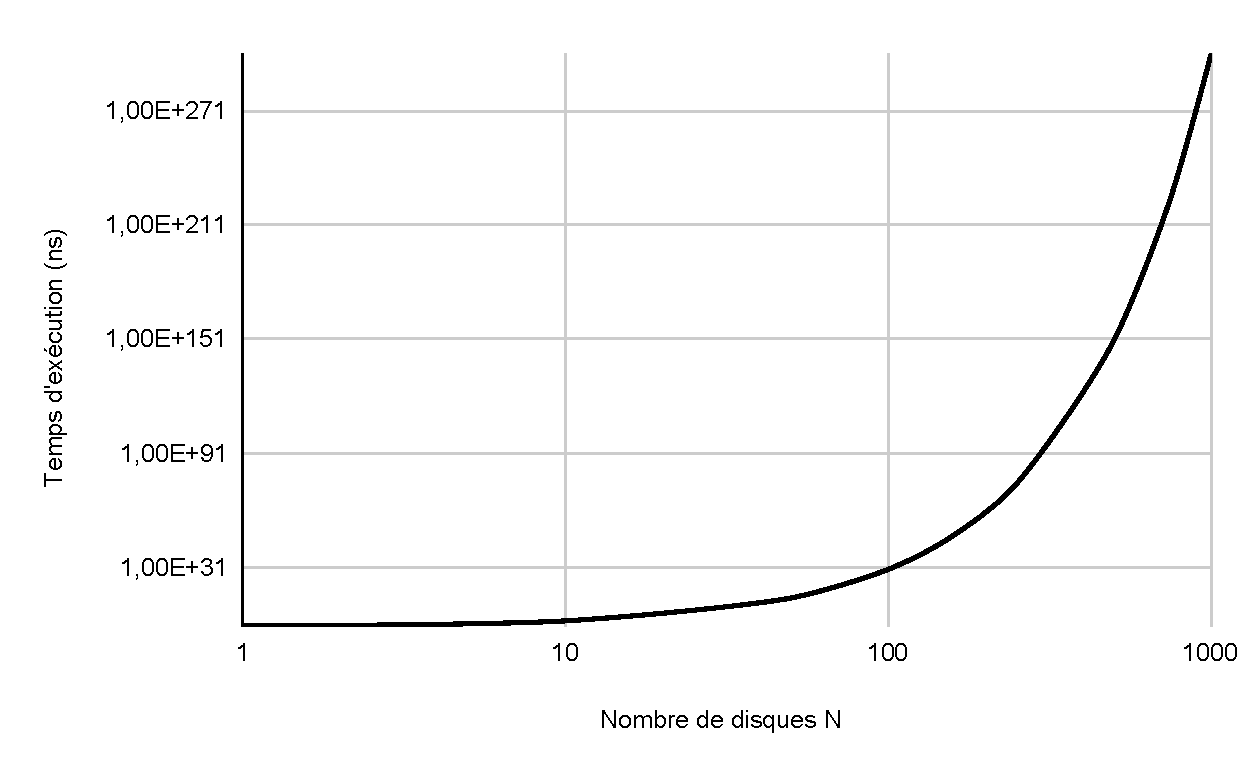
\includegraphics[scale=0.6]{./ressources/temps_execution_th_algo_reso.pdf}
        \caption{Temps d'exécution théorique de l'algorithme de résolution}
    \label{fig:temps_exec_th_algo_reso}
\end{figure} 

Depuis le graphe, nous observons que le temps d'exécution évolue de manière exponentielle selon le nombre de disques de départ. Il atteint rapidement des temps d'exécution incommensurables le rendant inexploitable.

\paragraph{Complexité spatiale}
L'algorithme exploite une matrice $3 * n$ tel que $n$ est le nombre de disques. Chaque disque est représenté par un entier de taille $4$ octets. De plus, la taille de la représentation est statique au cours de l'exécution. Par conséquent, la complexité spatiale est égale à $4 * 3 * n$ octets donc de l'ordre de $\mathcal{O}(n)$.
\par
Cependant, l'algorithme récursif fait au maximum $n$ appels récursifs (le nombre maximum d'appels est le nombre maximum de disques pouvant être déplacés à la fois). L'adresse de retour étant stockée sur $8$ octets, la taille maximale de la pile d'appel de fonctions exploitée est donc égale à $8 * n$ octets qui est de l'ordre de $\mathcal{O}(n)$.
\par
La complexité spatiale totale est donc de l'ordre de $\mathcal{O}(n)$.

\section{Complexité théorique de l'algorithme de vérification}
\paragraph{Complexité temporelle}
La complexité temporelle de l'algorithme de vérification est linéaire et elle est égale à $n \cong \mathcal{O}(n)$, car l'algorithme parcourt la tour d'arrivée et vérifie si les disques sont bien rangés dans le bon ordre.
\par
Le tableau suivant représente les temps d'exécution théorique en nanoseconde de l'algorithme de vérification selon la variation de la taille du problème (le nombre de disques) :

\small
\begin{center}
    \begin{tabular}{| c | c | c | c | c | c | c | c | c | c | c | c | c |}
        \hline
        N & 1 & 10 & 50 & 100 & 150 & 250 & 500 & 750 & 1000\\
        \hline
        t(ns) & 1 & 10 & 50 & 100 & 150 & 250 & 500 & 750 & 1000\\
        \hline
    \end{tabular}
\end{center}

La figure suivante (voir Figure \ref{fig:temps_exec_th_algo_verification}) représente l'évolution du temps d'exécution théorique selon le nombre de disques :

\begin{figure}[H]
    \centering
        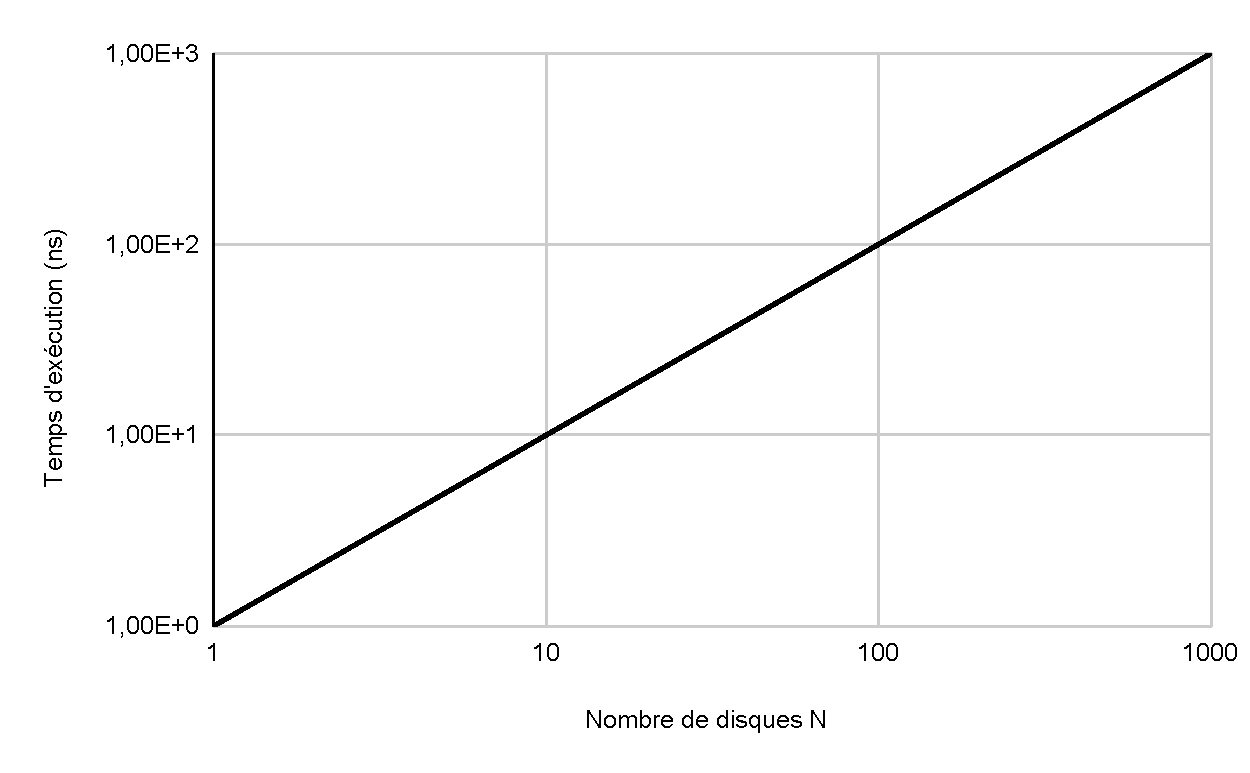
\includegraphics[scale=0.6]{./ressources/temps_execution_th_algo_verification.pdf}
        \caption{Temps d'exécution théorique de l'algorithme de vérification}
    \label{fig:temps_exec_th_algo_verification}
\end{figure} 

Depuis le graphe, nous observons que le temps d'exécution évolue avec une tendance linéaire avec l'augmentation du nombre de disques.

\paragraph{Complexité spatiale}
La complexité spatiale de l'algorithme de vérification est égale à la taille de la matrice plus l'indice de la tour cible qui est un entier, c.à.d. $3 * n + 4$ octets donc de l'ordre $\mathcal{O}(n)$.


\section{Expérimentation}

\subsection{Algorithme de résolution}

Le tableau suivant représente les temps d'exécution en nanoseconde de l'algorithme de résolution récursif selon la variation du nombre de disques.\\
\small
\begin{center}
    \begin{tabular}{| c | c | c | c | c | c | c | c |}
        \hline
        N & 3 & 5 & 7 & 10 & 15 & 20 & 25\\
        \hline
        t1(ns) & 663 & 2029 & 7829 & 59701 & 2168020 & 90192200 & 3190280000\\
        \hline
        t2(ns) & 595 & 2099 & 8018 & 60986 & 2648340 & 88261800 & 3188540000\\
        \hline
        t3(ns) & 642 & 2118 & 11230 & 62336 & 2206080 & 89520400 & 3176230000\\
        \hline
        t4(ns) & 597 & 2085 & 8118 & 61247 & 2211980 & 89318100 & 3179730000\\
        \hline
        t5(ns) & 596 & 2021 & 7724 & 61253 & 2168540 & 88693300 & 3187330000\\
        \hline
        t6(ns) & 882 & 2042 & 8044 & 61308 & 2275150 & 88450100 & 3175950000\\
        \hline
        t7(ns) & 867 & 2067 & 7977 & 63335 & 2258050 & 88788800 & 3181730000\\
        \hline
        t8(ns) & 615 & 2059 & 8085 & 63063 & 2301650 & 88529200 & 3178430000\\
        \hline
        t9(ns) & 593 & 2077 & 7942 & 60909 & 2211830 & 88074100 & 3176490000\\
        \hline
        t10(ns) & 619 & 2182 & 7955 & 61240 & 2221290 & 89301200 & 3182450000\\
        \hline
        moyenne(ns) & 667 & 2078 & 8292 & 61538 & 2267093 & 88912920 & 3181716000\\
        \hline
    \end{tabular}
\end{center}
\normalsize

\par
La figure suivante (voir Figure \ref{fig:temps_exec_algo_reso}) représente l'évolution du temps d'exécution selon le nombre de disques.

\begin{figure}[H]
    \centering
        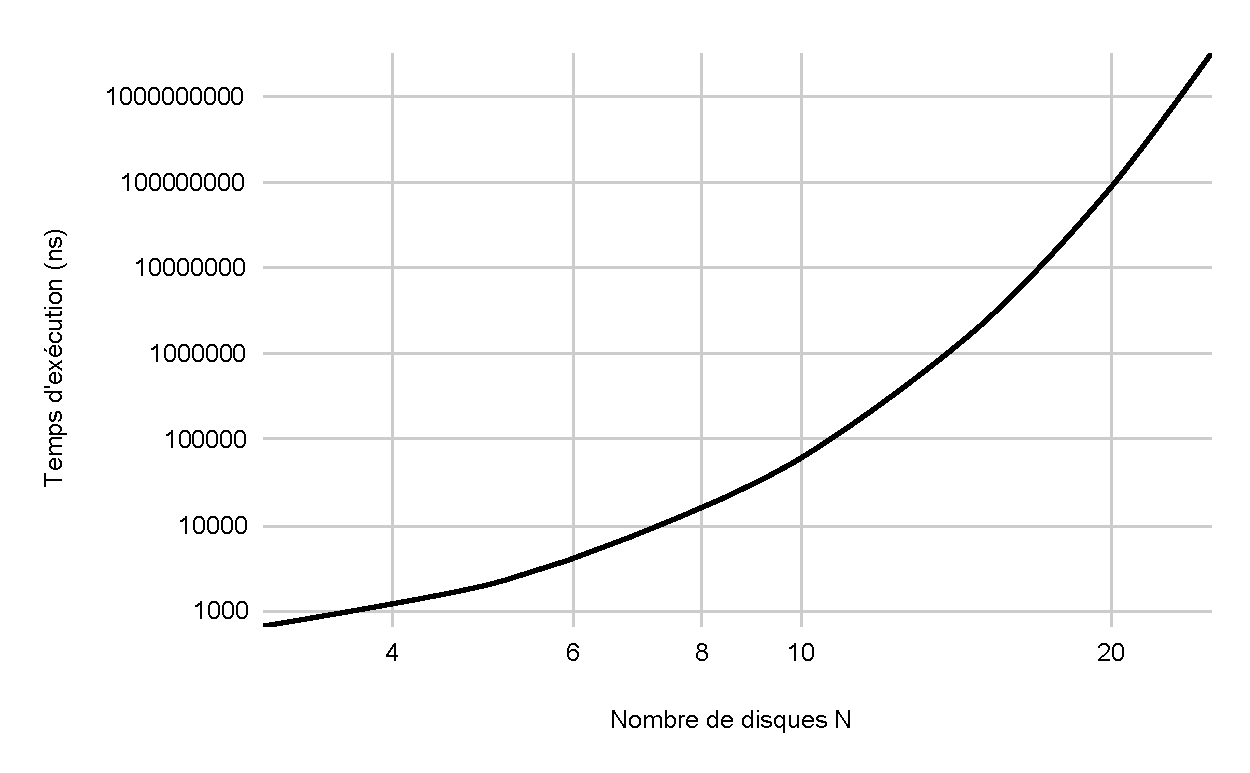
\includegraphics[scale=0.6]{./ressources/temps_execution_algo_reso.pdf}
        \caption{Temps d'exécution de l'algorithme de résolution}
    \label{fig:temps_exec_algo_reso}
\end{figure}
\par
Depuis la figure \ref{fig:temps_exec_algo_reso}, nous remarquons bien que le temps d'exécution de l'algorithme de résolution est exponentiel, conforme à la complexité de $\mathcal{O}(2^{n})$.

\subsection{Algorithme de génération de solution}
Cet algorithme fait au minimum $2^{n} - 1$ itérations, qui est équivalent au nombre d'étapes de la solution. Si l'algorithme génère à une étape un déplacement non autorisé, ce déplacement est rejeté et un autre est généré (si à son tour il n'est pas autorisé en génère un autre et ainsi de suite). Donc il est de complexité $\mathcal{O}(2^{n})$.
\par
Le tableau suivant représente les temps d'exécution en nanoseconde de l'algorithme de génération de solution pour le problème des tours de hanois selon la variation du nombre de disques.\\
\small
\begin{center}
    \begin{tabular}{| c | c | c | c | c | c | c | c |}
        \hline
        N & 3 & 5 & 7 & 10 & 15 & 20 & 25\\
        \hline
        t1(ns) & 16484 & 25099 & 73290 & 304737 & 11255800 & 401042000 & 14478900000\\
        \hline
        t2(ns) & 13480 & 23469 & 72592 & 310506 & 11503700 & 402620000 & 14470300000\\
        \hline
        t3(ns) & 15804 & 22381 & 70229 & 321948 & 11607800 & 401610000 & 14440400000\\
        \hline
        t4(ns) & 16334 & 24410 & 69875 & 312012 & 11348400 & 401075000 & 14418900000\\
        \hline
        t5(ns) & 15780 & 23887 & 79824 & 329052 & 11008400 & 402276000 & 14439500000\\
        \hline
        t6(ns) & 14275 & 21296 & 72074 & 321122 & 11444300 & 402046000 & 14443800000\\
        \hline
        t7(ns) & 13965 & 30082 & 52879 & 309217 & 1,17E+07 & 405221000 & 14440000000\\
        \hline
        t8(ns) & 14042 & 22535 & 62667 & 310238 & 1,14E+07 & 405030000 & 14471900000\\
        \hline
        t9(ns) & 13832 & 22679 & 49077 & 311514 & 11376700 & 405483000 & 14419800000\\
        \hline
        t10(ns) & 15764 & 22572 & 69374 & 311673 & 11215200 & 402717000 & 14449700000\\
        \hline
        moyenne(ns) & 14976 & 23841 & 67188 & 314202 & 11386730 & 402912000 & 14447320000\\
        \hline
    \end{tabular}
\end{center}
\normalsize
\par
La figure suivante (voir Figure \ref{fig:temps_exec_algo_generation}) représente l'évolution du temps d'exécution selon le nombre de disques.

\begin{figure}[H]
    \centering
        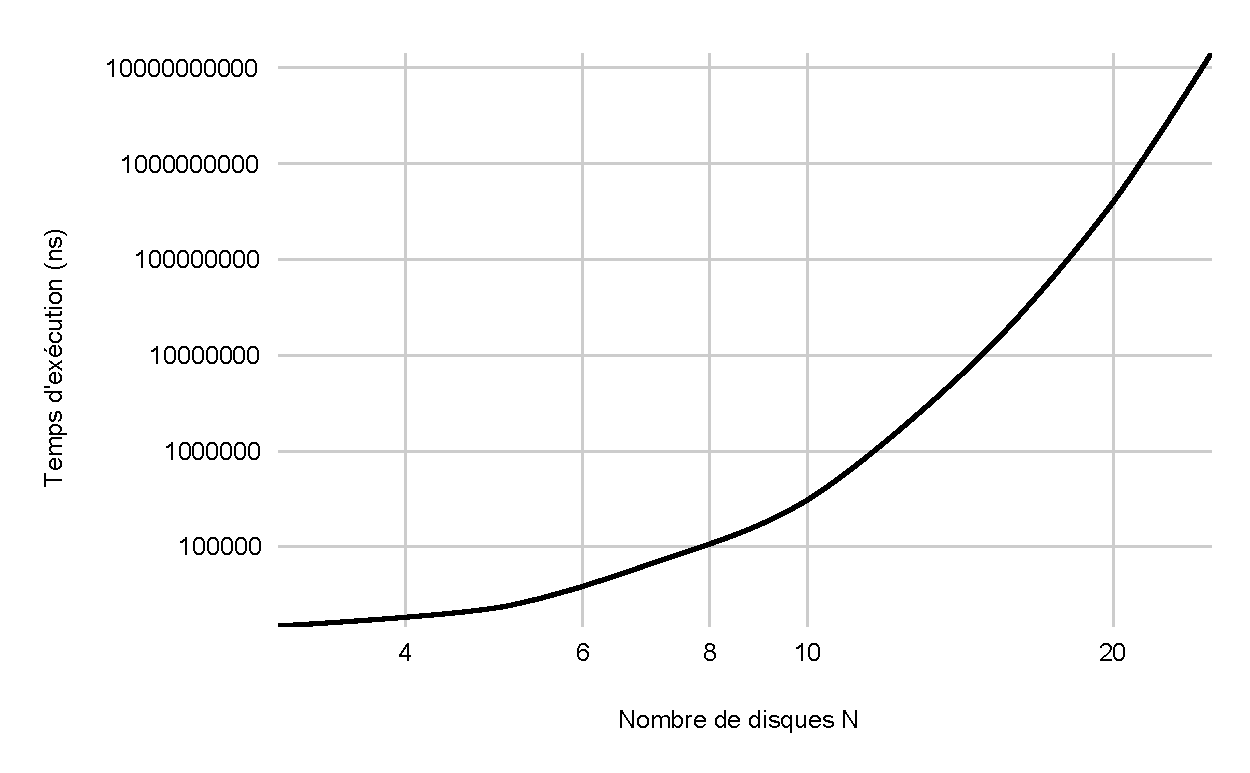
\includegraphics[scale=0.6]{./ressources/temps_execution_algo_generation.pdf}
        \caption{Temps d'exécution de l'algorithme de génération de solution}
    \label{fig:temps_exec_algo_generation}
\end{figure}
\par
Depuis la figure \ref{fig:temps_exec_algo_generation}, nous remarquons bien que le temps d'exécution de l'algorithme de résolution est exponentiel, conforme à la complexité de $\mathcal{O}(2^{n})$. Cependant, les temps d'exécution sont bien plus élevés que ceux de l'algorithme de résolution, car même si l'algorithme de génération fait $2^{n} - 1$ itération, certains déplacements sont rejetés.

\subsection{Algorithme de vérification de solution}
Le tableau suivant représente les temps d'exécution en nanoseconde de l'algorithme de vérification de solution pour le problème des tours de hanois selon la variation du nombre de disques.\\
\small
\begin{center}
    \begin{tabular}{| c | c | c | c | c | c | c | c |}
        \hline
        N & 3 & 5 & 7 & 10 & 15 & 20 & 25\\
        \hline
        t1(ns) & 71 & 61 & 113 & 80 & 75 & 146 & 182\\
        \hline
        t2(ns) & 61 & 68 & 111 & 68 & 77 & 94 & 61\\
        \hline
        t3(ns) & 66 & 95 & 66 & 80 & 143 & 84 & 156\\
        \hline
        t4(ns) & 68 & 68 & 82 & 66 & 101 & 86 & 143\\
        \hline
        t5(ns) & 76 & 75 & 97 & 108 & 65 & 141 & 197\\
        \hline
        t6(ns) & 57 & 67 & 81 & 110 & 64 & 104 & 179\\
        \hline
        t7(ns) & 58 & 90 & 77 & 104 & 180 & 148 & 91\\
        \hline
        t8(ns) & 74 & 73 & 70 & 78 & 137 & 147 & 102\\
        \hline
        t9(ns) & 78 & 75 & 74 & 117 & 105 & 126 & 105\\
        \hline
        t10(ns) & 60 & 66 & 68 & 80 & 68 & 78 & 164\\
        \hline
        moyenne(ns) & 67 & 74 & 84 & 89 & 102 & 115 & 138\\
        \hline
    \end{tabular}
\end{center}
\normalsize
\par
La figure suivante (voir Figure \ref{fig:temps_exec_algo_verification}) représente l'évolution du temps d'exécution selon le nombre de disques.

\begin{figure}[H]
    \centering
        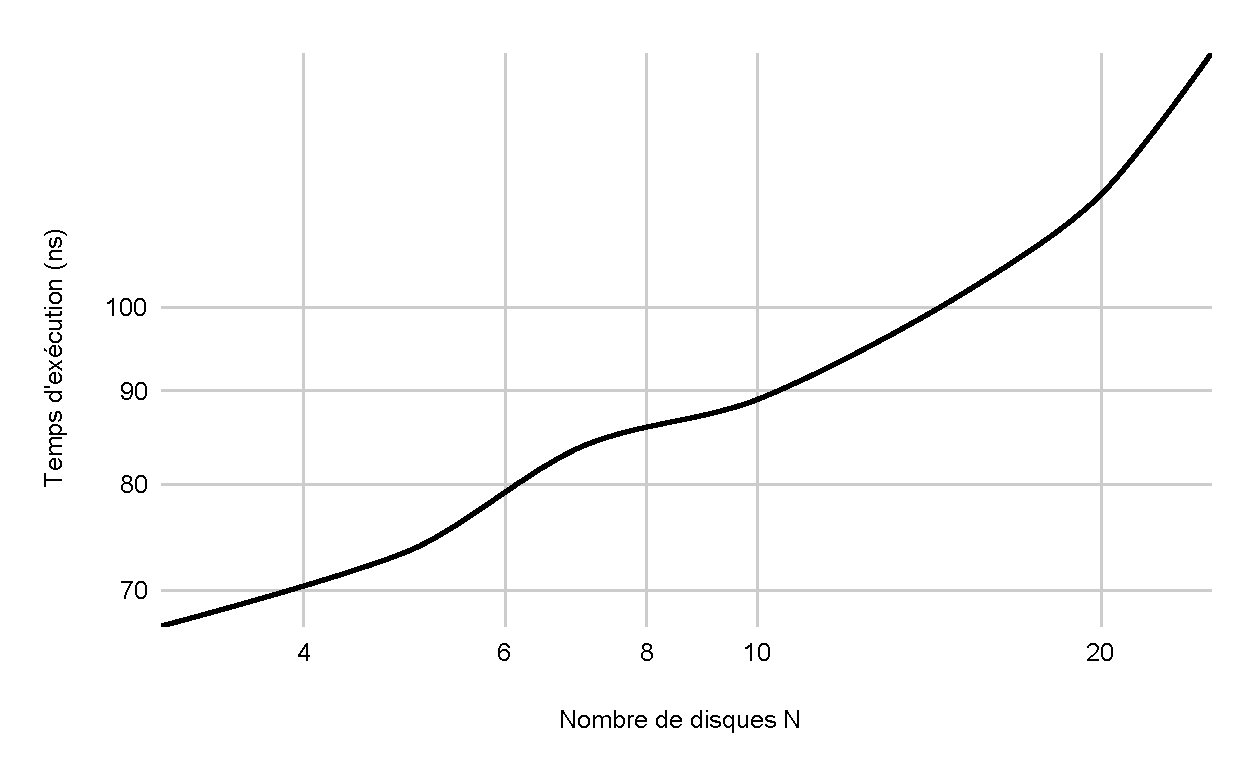
\includegraphics[scale=0.6]{./ressources/temps_execution_algo_verification.pdf}
        \caption{Temps d'exécution de l'algorithme de vérification de solution}
    \label{fig:temps_exec_algo_verification}
\end{figure}
\par
Depuis la figure \ref{fig:temps_exec_algo_verification}, nous observons une trajectoire presque linéaire, qui est représentative de la complexité $\mathcal{O}(n)$. Les fluctuations sont dûes au nombre de disques relativement bas.

\paragraph{Discussion des résultats}
On constate que la complexité de l'algorithme de résolution pour le problème des tours de hanoi évolue bien de manière exponentielle comme l'a montré l'étude expérimentale. Le temps d'exécution pour une instance du problème de 20 disques est de l'ordre de dizaine de secondes, celle avec 30 disques dépasse les quinzaines de minutes. Avec de tels résultats, il est clair que l'exploitation effective de ce genre de complexités est inenvisageable, voire impossible.
\par
Quant à l'algorithme de vérification, il a une simple complexité linéaire. Il ne fait que vérifier l'état de la dernière tour, les déplacements quant à eux, sont supposés corrects et valides par l'algorithme de génération de solution.
